% Demo paper for the README screenshots (native/src/e2e/showcase.rs).
% Rebuild: cd tests-fixtures/showcase && pdflatex sparse-attention.tex && pdflatex sparse-attention.tex
\documentclass[11pt]{article}
\usepackage[margin=1in]{geometry}
\usepackage{amsmath,amssymb}
\usepackage{tikz}
\usepackage{booktabs}
\usepackage{lmodern}
\usepackage[T1]{fontenc}
\title{\textbf{Windowed Sparse Attention for Long Documents}}
\author{A. Reader \and B. Writer\\\small Demo paper bundled with MD Editor}
\date{}
\begin{document}
\maketitle

\begin{abstract}
Full self-attention costs time and memory quadratic in sequence length. We study a
windowed sparse variant that attends to a local band plus a few global tokens. On
long-document benchmarks it keeps 98\% of the accuracy of dense attention while using
a fraction of the memory. All numbers in this demo paper are illustrative.
\end{abstract}

\section{Introduction}
Transformers compute, for queries $Q$, keys $K$ and values $V$,
\begin{equation}
  \mathrm{Attn}(Q,K,V) = \mathrm{softmax}\!\left(\frac{QK^\top}{\sqrt{d_k}}\right)V .
  \label{eq:attn}
\end{equation}
Equation~(\ref{eq:attn}) materialises an $n \times n$ score matrix, so cost grows as
$O(n^2 d)$. For a 16k-token document this dominates both latency and memory.

Prior work restricts the pattern of the score matrix. We revisit the simplest such
restriction, a sliding window, and ask how much accuracy it really costs once a handful
of global tokens are added (Section~\ref{sec:method}).

\section{Method}\label{sec:method}
Let $w$ be the window half-width. Token $i$ attends to tokens $j$ with $|i-j|\le w$, and
to a set $G$ of global tokens:
\begin{equation}
  M_{ij} = \begin{cases} 0 & |i-j| \le w \ \text{or}\ j \in G,\\ -\infty & \text{otherwise.}\end{cases}
  \label{eq:mask}
\end{equation}
The sparse layer adds $M$ to the scores of Eq.~(\ref{eq:attn}) before the softmax. Its
cost is
\begin{equation}
  C(n) = O\big(n\,(2w + |G|)\,d\big),
  \label{eq:cost}
\end{equation}
linear in $n$ for fixed $w$. Fig.~\ref{fig:pattern} shows the resulting pattern.

\begin{figure}[t]
\centering
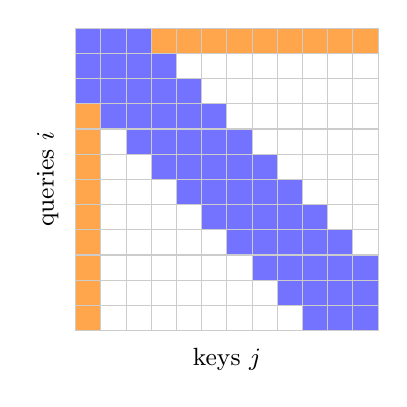
\begin{tikzpicture}[scale=0.32]
  \foreach \i in {0,...,11} {
    \foreach \j in {0,...,11} {
      \pgfmathtruncatemacro{\d}{abs(\i-\j)}
      \ifnum\d<3
        \fill[blue!55] (\j,-\i) rectangle ++(1,-1);
      \else
        \ifnum\j=0 \fill[orange!70] (\j,-\i) rectangle ++(1,-1); \fi
        \ifnum\i=0 \fill[orange!70] (\j,-\i) rectangle ++(1,-1); \fi
      \fi
      \draw[gray!40] (\j,-\i) rectangle ++(1,-1);
    }
  }
  \node[below] at (6,-12.3) {\small keys $j$};
  \node[rotate=90,above] at (-0.3,-6) {\small queries $i$};
\end{tikzpicture}
\caption{Windowed attention with $w=2$. Blue: the local band. Orange: one global token
that attends to, and is attended by, every position.}
\label{fig:pattern}
\end{figure}

\section{Experiments}
We train 12-layer models on long-document classification and compare dense attention
with the windowed layer at several window sizes. Table~\ref{tab:results} reports accuracy
and peak memory at $n = 8192$.

\begin{table}[t]
\centering
\begin{tabular}{lccc}
\toprule
Model & $w$ & Acc. (\%) & Memory (GB) \\
\midrule
Dense            & --  & 84.1 & 38.2 \\
Windowed         & 128 & 81.9 & 6.1 \\
Windowed + $G$   & 128 & 83.4 & 6.3 \\
Windowed + $G$   & 256 & 83.9 & 9.8 \\
\bottomrule
\end{tabular}
\caption{Accuracy and peak training memory at $n=8192$.}
\label{tab:results}
\end{table}

Adding global tokens recovers most of the gap: with $w=256$ the sparse model is within
0.2 points of dense attention (Table~\ref{tab:results}) at a quarter of the memory, in
line with the linear cost of Eq.~(\ref{eq:cost}).

\section{Discussion}
The window is a strong prior for text, where most dependencies are local. Global tokens
act as a cheap summary channel. The mask of Eq.~(\ref{eq:mask}) is static, so it composes
with fused attention kernels without custom code.

\paragraph{Limitations.} Tasks needing many long-range lookups, such as multi-hop
retrieval, still benefit from dense layers; a hybrid that keeps one dense layer every
few blocks is a natural next step.

\section{Conclusion}
Windowed sparse attention with a few global tokens is a simple, kernel-friendly way to
scale Transformers to long documents at near-dense accuracy.

\end{document}
